\begin{frame}{RTM Design Space Exploration}
  \begin{itemize}
  \item timing closure, build time vs parallelism
  \end{itemize}
  \begin{figure}[!h]
    \centering
    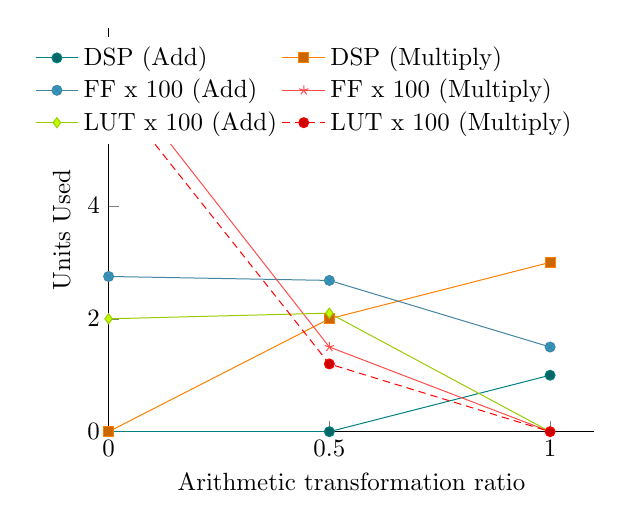
\begin{tikzpicture}[scale=0.9]
      \begin{axis}[
        cycle list name=exotic,
        xmin=0,
        ymin=0,
        axis y line*=left,
        axis x line* =bottom,
        xlabel=Arithmetic transformation ratio,
        ylabel=Units Used,
        xtick={0, 0.5, 1},
        legend columns=2,
        legend entries={
          DSP (Add),
          DSP (Multiply),
          FF x 100 (Add),
          FF x 100 (Multiply),
          LUT x 100 (Add),
          LUT x 100 (Multiply),
        },
        legend style={
          draw=none,
          cells={anchor=west}
        }
        ]
        \addplot coordinates {
          (0, 0)
          (0.5, 0)
          (1, 1)
        };
        \addplot coordinates {
          (0, 0)
          (0.5, 2)
          (1, 3)
        };
        \addplot coordinates {
          (0, 2.75)
          (0.5, 2.68)
          (1, 1.50)
        };
        \addplot coordinates {
          (0, 6.5)
          (0.5, 1.5)
          (1, 0)
        };
        \addplot coordinates {
          (0, 2)
          (0.5, 2.1)
          (1, 0)
        };
        \addplot coordinates {
          (0, 6.13)
          (0.5, 1.2)
          (1, 0)
        };
      \end{axis}
    \end{tikzpicture}
  \end{figure}
\end{frame}

\begin{frame}{4. Evaluation}
  \frametitle{RTM Word Length Exploration}
  \begin{itemize}
  \item accuracy vs resource usage: double parallelism
  \end{itemize}
  \begin{figure}
    \centering
    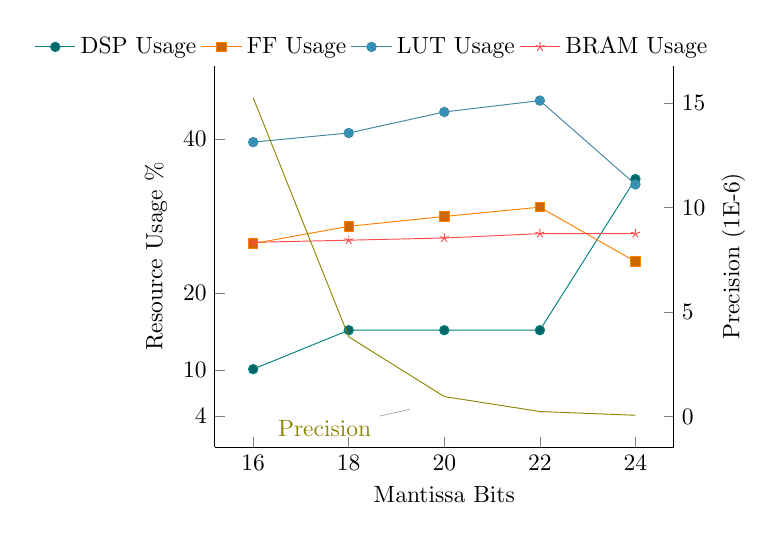
\begin{tikzpicture}[scale=0.85]
      \begin{axis}[
        cycle list name=exotic,
        ymin=0,
        axis y line*=left,
        axis x line*=bottom,
        xlabel=Mantissa Bits,
        ylabel=Resource Usage \%,
        xtick=data,
        ytick={4, 10, 20, 40, 50, 70, 80, 100},
        legend columns=4,
        legend entries={
          DSP Usage,
          FF Usage,
          LUT Usage,
          BRAM Usage},
        legend style={
          draw=none,
          anchor=east,
          at={(1.1, 1.05)}
        }
        ]
        \addplot coordinates {
          (24, 34.82)
          (22, 15.18)
          (20, 15.18)
          (18, 15.18)
          (16, 10.12)
        };
        \addplot coordinates {
          (24, 24.09)
          (22, 31.17)
          (20, 29.96)
          (18, 28.68)
          (16, 26.44)
        };
        \addplot coordinates {
          (24, 34.13)
          (22, 45.02)
          (20, 43.54)
          (18, 40.81)
          (16, 39.62)
        };
        \addplot coordinates {
          (24, 27.73)
          (22, 27.73)
          (20, 27.16)
          (18, 26.88)
          (16, 26.60)
        };
      \end{axis}
      \begin{axis}[
        ylabel=Precision (1E-6),
        axis y line*=right,
        axis x line=none,
        ]
        \addplot[color=olive] coordinates {
          (16, 15.2585)
          (18, 3.8146)
          (20, 0.9536)
          (22, 0.2394)
          (24, 0.0596)
        } node [pos=0.8,pin={190:Precision},inner sep=20pt] {};
      \end{axis}
    \end{tikzpicture}
  \end{figure}
\end{frame}

\begin{frame}{4. Evaluation}
  \frametitle{RTM Parallelism}
  \begin{itemize}
  \item performance vs build time, identify resource bottlenecks
  \end{itemize}
  \begin{figure}
    \centering
    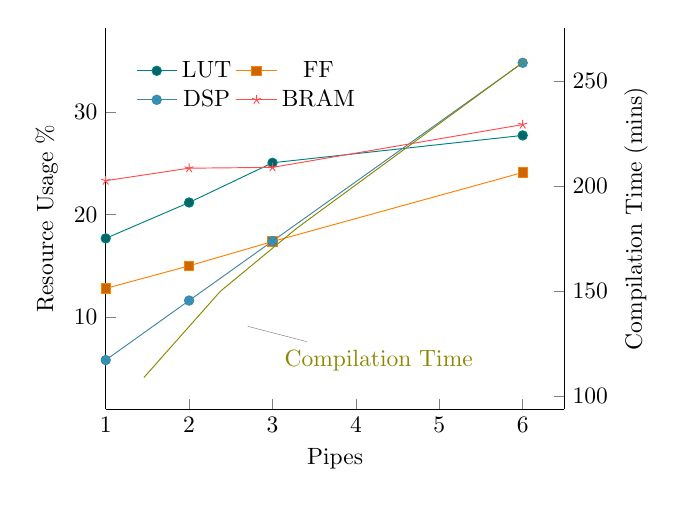
\begin{tikzpicture}[scale=0.85]
      \begin{axis}[
        cycle list name=exotic,
        xmin=1,
        ymin=1,
        xlabel=Pipes,
        ylabel=Resource Usage \%,
        axis x line* =bottom,
        axis y line* = left,
        legend columns=2,
        legend entries={
          LUT,
          FF,
          DSP,
          BRAM,
        },
        legend style={
          draw=none,
          at={(0.05,0.85) },
          anchor=west
        }
        ]
        \addplot coordinates {
          (1, 17.68)
          (2, 21.18)
          (3, 25.06)
          (6, 27.73)
        };
        \addplot coordinates {
          (1, 12.79)
          (2, 15.00)
          (3, 17.37)
          (6, 24.11)
        };
        \addplot coordinates {
          (1, 5.80)
          (2, 11.61)
          (3, 17.41)
          (6, 34.82)
        };
        \addplot coordinates {
          (1, 23.31)
          (2, 24.53)
          (3, 24.61)
          (6, 28.79)
        };
      \end{axis}
      \begin{axis}[
        ylabel=Compilation Time (mins),
        axis y line*=right,
        axis x line=none,
        ]
        \addplot[color=olive] coordinates {
          (1, 109)
          (2, 150)
          (3, 180)
          (6, 260)
        }  node [pos=0.2,pin={340:Compilation Time},inner sep=20pt] {};
      \end{axis}
    \end{tikzpicture}
  \end{figure}

\end{frame}

\begin{frame}{4. Evaluation}
  \frametitle{RTM Performance}

  {\scriptsize

    \begin{table}
      \renewcommand{\arraystretch}{1.5}
      \hspace*{-8pt}\makebox[\linewidth][c]{
        \begin{tabular}{c|p{0.55cm}|p{0.5cm}|p{0.6cm}|p{0.6cm}|p{0.65cm}|p{0.65cm}|p{0.65cm}|p{0.75cm}|p{0.65cm}}
          & \textbf{CPU} & \textbf{GPU} [1] & \textbf{GPU} [2] & \textbf{GPU} [3] & \textbf{FPGA} [4]& \textbf{FPGA} [5] \ & \textbf{FPGA} & \textbf{FPGA D\footnote{D = Dynamic (i.e. using run-time reconfiguration)}} [5] & \textbf{FPGA D} \\
          \hline \hline
          Freq.(GHz) & 2.7          & 1.15         &    1.15          &   1.15           &    0.1           & 0.1                 & 0.1                 & 0.1                 & 0.1                 \\
          Time (s)   & 1458         & 52           &    --          &     --         &    --           & 18                  & 18.3                & 13.4                & 13.6                \\
          GFLOP/s    & 0.9          & 51.2         &    36          &     64.5         &    35.8          & 68.0                & 66.8                & 91.6                & 90.2                \\
          Speed-up(X)   & 1           & 56.8        &   40          &     71.6         &     39.7          & 76.4               & \textbf{74.22}     & 102.9              & \textbf{101.3}     \\
          Power (W)  & 185          & --        &    461          &      --        &         --      & 129                 & 126                 & 128                 & 125                 \\
          Efficiency & 4.9          & --        &    78          &       --       &    --           & 527.1               & 527.7               & 715.6               & 721.6               \\
          Eff. Gains & 1           & --        &    15.9          &        --      & --            & 107.5              & \textbf{107.0}     & 146.0             & \textbf{147.1}     \\
        \end{tabular}
      }
    \end{table}

  }

  {\footnotesize
  \begin{columns}[t]
    \begin{column}{.5\textwidth}
      \begin{itemize}
      \item [1] Phillips, Everett, IPDPS, 2010
      \item [2] Datta, Kaushik, ICS, 2008
      \item [3] Yang, Yang, JCST, 2008
      \end{itemize}
    \end{column}
    \begin{column}{.6\textwidth}
    \begin{itemize}
    \item [4] Arraya-Polo, Mauricio, TPDS, 2011
    \item [5] Niu, Xinyu, FPL, 2012
    \end{itemize}
    \end{column}
  \end{columns}
}

\end{frame}

\begin{frame}{4. Evaluation}
  \frametitle{Wider Benchmark Results}
  Comparing manual MaxCompiler designs to FAST designs:
  {\footnotesize
    \begin{table}
      \renewcommand{\arraystretch}{1.5}
      \begin{tabular}{l|c|c|c|c|c}
        \textbf{Kernel} & \textbf{Size} & \textbf{Reduction} & \textbf{API Calls} & \textbf{Performance}              & \textbf{Resource}
        \\
        \hline\hline
        CmdRead       & 48 & 43 \%               & 4.33                     & \multirow{2}{1.5cm}{$ > 75\%$}        & \multirow{6}{1.5cm}{$\approx 100\%$} \\
        CmdWrite      & 54  & 31 \%              & 4.13                     &                                   &                              \\
        \cline{1-4}
        RTM            & 231 & 27 \%              & 10                       & \multirow{5}{1.5cm}{$ \approx 100\%$} &                              \\
        SGSmooth      & 60 & 45 \%              & 14                       &                                   &                              \\
        SGDiff       & 58 & 42 \%              & 14                       &                                   &                              \\
        Black-Scholes & 56  & 60 \%               & 5.5                      &                                   &                              \\
        \cline{5-5}
        Ad Prediction & 94 & 40 \%             & 16                       &                                   &    $ \approx 117 \% $                          \\
        Bitonic Sort & 102 & 38 \%             & 12                    &                                   &    $ \approx 100 \% $                          \\
      \end{tabular}
    \end{table}}

\end{frame}